\chapter{Realization}

In the following chapter, we describe the realization of the software system. In section \ref{sec:structure}, we give an overview of the different components and how they interact with each other.

\section{Structure}\label{sec:structure}

The system consists of three major components: the \emph{Bot Service}, the \emph{Mensa Service} and the \emph{MobSOS CCA system}. The Bot Service communicates with the user through a \emph{Chat Platform}, called Slack. The bot will receice messages from the user and will respond to them through chat.

The Bot Service communicates with the \emph{Mensa Service} in order to get the menu for the canteen. Furthermore the bot service can send requests to the Mensa service, telling it to add, or modify, reviews. The reviews are stored inside a las2peer database.

The MobSOS CCA system can access the reviews, which are stored inside the database, in order to incprporate this data into the success model. The MobSOS CCA system also is provided monitoring messages by the bot service, which logs incoming requests. Those monitoring messages can also be included into the success model. Mediabase data, which contains data from reviews, made outside of the las2peer system, is also included into the success model.

The Bot Service communicates with the MobSOS CCA system in order to retrieve visualizations of the success model.
\begin{figure}[h!]
    \centering
    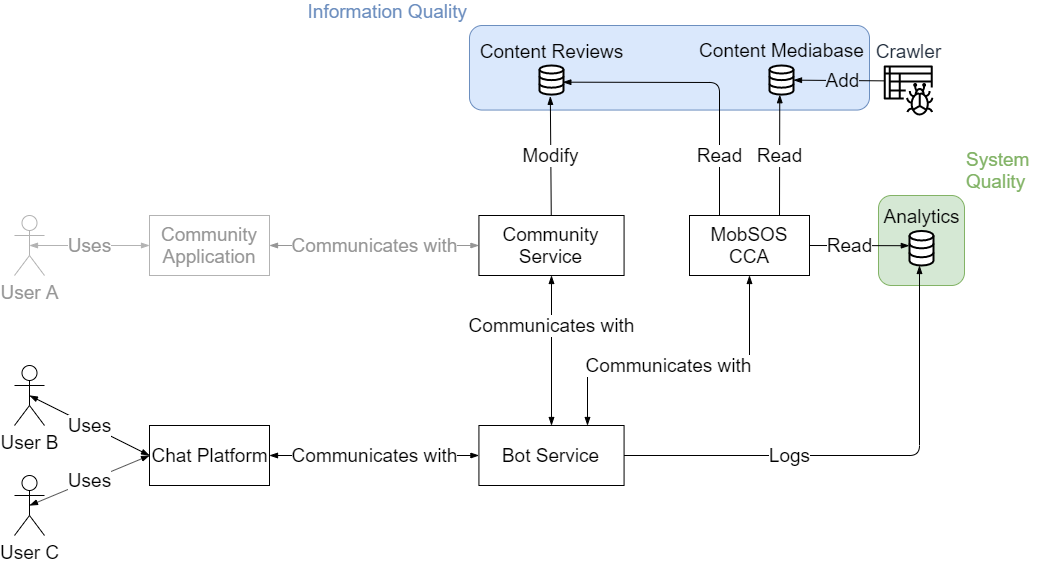
\includegraphics[width=0.9\linewidth]{realization/Component_Diagramm.png}
\end{figure}

\section{Changes to Core Components}

The Social Bot Framework needs to be extended, such that the bot is able to listen to specific mentions in group chats.